% !TeX root = ../mat_mod2.tex

\subsection{
  Условие предшествования
}
\label{sect:1.3.2}

Это условие накладывает ограничения на порядок вырезки сегментов
$ I = (i_1, i_2, \,\dots, i_K)$.
Ограничения на порядок их резки обусловлены особенностями
технологии и оборудования листовой резки с ЧПУ,
которые не позволяют после вырезки внешнего контура точно
позиционировать инструмент для вырезки внутренних контуров,
поскольку деталь после вырезки внешнего контура может
изменить свое положение на раскройном столе.
Это вызвано тем, что после вырезки внешнего контура
вырезанная деталь <<теряет>> связь с листом,
а для многих типов раскройных столов эта деталь
может даже изменить свое положение относительно плоскости листа
(упасть между статическими конструкциями раскройного стола).
При выборе последовательности контуров
необходимо придерживаться следующих правил.

{\it Правило 1}.
Если внешний контур имеет один или более внутренних контуров,
которые представляют собой границы отверстий в деталях,
то прежде, чем будет начата вырезка внешнего контура,
должны быть вырезаны все внутренние контуры.

{\it Правило 2}.
Если внутренний контур детали на раскройной карте
содержит внешний контур/контуры другой детали,
то сначала должна быть вырезана эта другая деталь
с соблюдением {\it Правила 1}.

Перечисленные правила и называются условием предшествования для перестановки
$ I = (i_1, i_2, \,\dots, i_K)$.
В терминах ее элементов условие означает следующее:
\begin{itemize}
  \item
  если в перестановке
  $ I = (i_1, i_2, \,\dots, i_K)$
  сегмент $i_k$
  содержит внешний контур,
  то все соответствующие внутренние контуры должны содержаться в сегментах,
  предшествующих сегменту $i_k$
  в перестановке;
  \item
  если в перестановке
  $ I = (i_1, i_2, \,\dots, i_K)$
  сегмент $i_k$
  содержит  внутренний контур,
  который на раскройной карте содержит внутри внешний контур,
  соответствующий другому объекту
  $A_l$
  $(l=1,2, \,\dots, n)$,
  то этот внешний контур должен быть вырезан в сегментах,
  предшествующих сегменту $i_k$ в перестановке $I$.
\end{itemize}

Рис.~\ref{precedence}
иллюстрирует условие предшествования
при формировании маршрута резки для деталей,
содержащих внутренние контуры.

В соответствии с условиями предшествования резка контуров,
ограничивающих цветные области для четырех деталей на
рис.~\ref{precedence},
должна осуществляться в следующей последовательности.
\begin{enumerate}
  \item желтый, красный, синий, серый;
  \item	красный, синий, серый;
  \item	желтый, серый;
  \item желтый, серый.
\end{enumerate}

\begin{figure}[h]
  \begin{center}
  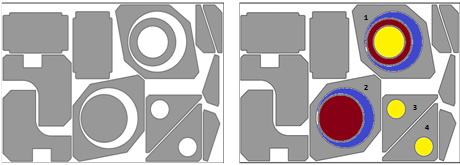
\includegraphics[width=0.9\textwidth]{precedence.png}
  \caption{Пример раскройной карты деталей, содержащих внутренние контуры}
  \label{precedence}
  \end{center}
\end{figure}

Условия предшествования и ограничения координат точек врезки
и точки выключения инструмента,
обусловленные деформацией материала при врезке,
имеют статический характер,
т. е. однозначно определяются спроектированной раскройной картой,
используемым для резки технологическим оборудованием
и свойствами раскраиваемого материала.
В терминах маршрута резки $ROUTE$
и его параметров
$M_0$, $M_1$, $S_1$, $M_1^*$, $M_2$, $S_2$, $M_2^*$, \,\dots, $M_K$, $S_K$, $M_K^*$,
$i_1$, $i_2$, \,\dots, $i_K$
технологическое ограничение
1) однозначно определяет допустимые геометрические области
$G_M$
и
$G_{M^*}$
для выбора точек врезки и точек выключения инструмента,
а технологическое ограничение
2) накладывает запрет на некоторые значения перестановки
$ I = (i_1, i_2, \,\dots, i_K)$
при формировании порядка резки сегментов.
При этом сформулированные требования не зависят от задаваемых параметров кортежа
$ROUTE$.

В отличие от этих двух технологических ограничений
следующий тип технологических требований устанавливает
дополнительные ограничения на выбор точки врезки и выбор
порядка резки сегментов на каждом шаге формирования маршрута резки
(т. е. при определении параметров очередного выбираемого сегмента)
в зависимости от того какие параметры маршрута резки были выбраны на предыдущих шагах.
Этот тип ограничений обусловлен геометрическими
искажениями материала при термической резке деталей.
